\section{Decomposition summary}
\label{app:decomp}

% GENERATED by make_paper_assets.py -- do not edit by hand.
\begin{table}[H]
\centering
\small
\begin{adjustbox}{max width=\columnwidth}
\begin{tabular}{lr}
\toprule
Quantity & Value \\
\midrule
Method--model pairs & 32 \\
Pairs reporting an improvement & 32/32 \\
\textbf{Median mechanical fraction} & \textbf{80.4\%} \\
Mean mechanical fraction & 75.5\% \\
Pairs $\ge$90\% mechanical & 14/32 \\
Pairs $\ge$75\% mechanical & 17/32 \\
Pairs where disposition \emph{worsened} & 7/32 \\
\textbf{Pairs where identified set widened} & \textbf{31/32} \\
Mean identified width, before & 0.21 \\
Mean identified width, after & 0.61 \\
\bottomrule
\end{tabular}
\end{adjustbox}
\caption{Decomposition of all 32 method--model pairs in Table 11(a) of
\citet{bae2025decap} (BBQ ambiguous split, four interventions $\times$ eight
models, each against its own \textsc{Base} row). The mechanical fraction is the
coverage component as a share of the reported change. Source numbers are
transcribed verbatim from the published table.}
\label{tab:decomposition}
\end{table}


% GENERATED by make_paper_assets.py -- do not edit by hand.
\begin{figure}[t]
\centering
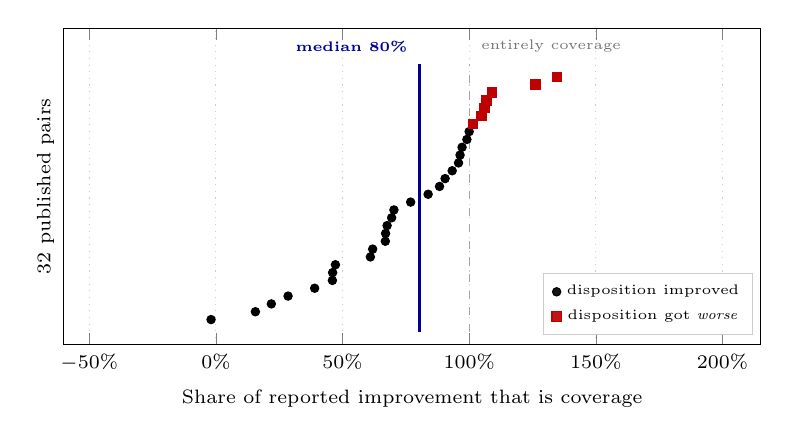
\begin{tikzpicture}
\begin{axis}[
  width=0.86\columnwidth, height=5.6cm,
  xmin=-60, xmax=215, ymin=-3.2, ymax=37.2,
  xtick={-50,0,50,100,150,200},
  xticklabels={$-$50\%,0\%,50\%,100\%,150\%,200\%},
  ytick=\empty,
  xlabel={Share of reported improvement that is coverage},
  ylabel={32 published pairs},
  tick label style={font=\scriptsize}, label style={font=\scriptsize},
  xmajorgrids, grid style={dotted, gray!40},
  legend style={at={(0.99,0.03)}, anchor=south east, font=\tiny,
                draw=gray!40, fill=white, fill opacity=0.92, text opacity=1},
  clip=false,
]
\draw[dashed, gray!70] (axis cs:100,-1.6) -- (axis cs:100,32.6);
\node[anchor=south west, font=\tiny, gray!90!black] at
  (axis cs:101,32.9) {entirely coverage};
\draw[thick, blue!60!black] (axis cs:80.4,-1.6) --
  (axis cs:80.4,32.6);
\node[anchor=south east, font=\tiny\bfseries, blue!60!black] at
  (axis cs:79.4,32.9) {median 80\%};
\addplot[only marks, mark=*, mark size=1.5pt, black]
  coordinates {(-1.9,0) (15.6,1) (21.9,2) (28.5,3) (39.0,4) (46.0,5) (46.1,6) (47.2,7) (61.0,8) (61.9,9) (66.9,10) (67.0,11) (67.6,12) (69.4,13) (70.3,14) (76.9,15) (83.8,16) (88.3,17) (90.5,18) (93.3,19) (95.8,20) (96.4,21) (97.2,22) (99.1,23) (100.0,24)};
\addlegendentry{disposition improved}
\addplot[only marks, mark=square*, mark size=1.7pt, red!75!black]
  coordinates {(101.6,25) (104.8,26) (106.0,27) (106.9,28) (109.0,29) (126.1,30) (134.6,31)};
\addlegendentry{disposition got \emph{worse}}
\end{axis}
\end{tikzpicture}
\caption{Every method--model pair in \citet{bae2025decap}'s ambiguous-split
table, sorted by the share of its reported bias-score improvement that is
coverage (the model abstaining more) rather than disposition (the model
actually preferring the stereotype less). Points beyond 100\% are pairs where
coverage over-explains the reported gain because disposition moved the wrong
way. The seven squares are pairs whose committed-answer bias \emph{worsened}
while the reported score improved.}
\label{fig:decomposition}
\end{figure}


% GENERATED by make_paper_assets.py -- do not edit by hand.
\begin{figure}[t]
\centering
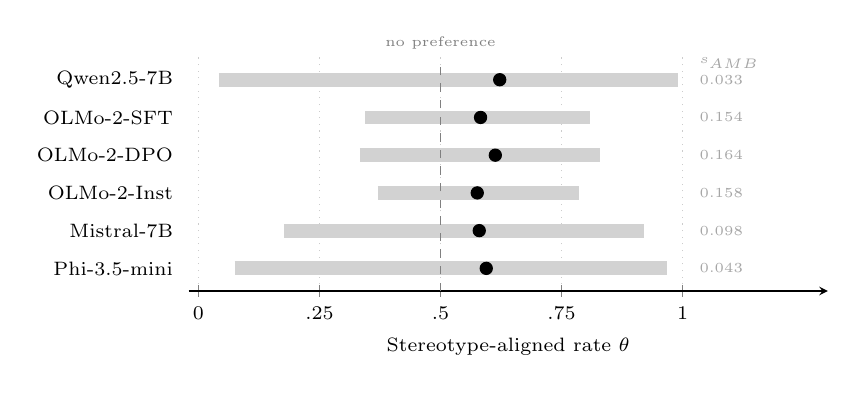
\begin{tikzpicture}
\begin{axis}[
  width=0.80\columnwidth, height=4.6cm,
  xmin=-0.02, xmax=1.30, ymin=0.4, ymax=6.7,
  xtick={0,0.25,0.5,0.75,1},
  xticklabels={0,.25,.5,.75,1},
  ytick={6,5,4,3,2,1},
  yticklabels={Qwen2.5-7B,OLMo-2-SFT,OLMo-2-DPO,OLMo-2-Inst,Mistral-7B,Phi-3.5-mini},
  xlabel={Stereotype-aligned rate $\theta$},
  tick label style={font=\scriptsize}, label style={font=\scriptsize},
  axis lines=left, y axis line style={draw=none}, ytick style={draw=none},
  xmajorgrids, grid style={dotted, gray!40},
  clip=false,
]
    \draw[line width=5pt, gray!35] (axis cs:0.0423,6) -- (axis cs:0.9905,6);
    \draw[line width=5pt, gray!35] (axis cs:0.3450,5) -- (axis cs:0.8086,5);
    \draw[line width=5pt, gray!35] (axis cs:0.3335,4) -- (axis cs:0.8303,4);
    \draw[line width=5pt, gray!35] (axis cs:0.3707,3) -- (axis cs:0.7869,3);
    \draw[line width=5pt, gray!35] (axis cs:0.1768,2) -- (axis cs:0.9209,2);
    \draw[line width=5pt, gray!35] (axis cs:0.0750,1) -- (axis cs:0.9682,1);
\addplot[only marks, mark=*, mark size=2.2pt, black] coordinates {
  (0.6223,6) (0.5827,5) (0.6132,4) (0.5759,3) (0.5800,2) (0.5945,1)};
\draw[dashed, gray] (axis cs:0.5,0.4) -- (axis cs:0.5,6.55);
\node[anchor=south, font=\tiny, gray] at (axis cs:0.5,6.55)
  {no preference};
\node[anchor=west, font=\tiny\bfseries, gray!70] at
  (axis cs:1.015,6.45) {$s_{\text{AMB}}$};
    \node[anchor=west, font=\tiny, gray!70] at (axis cs:1.015,6) {0.033};
    \node[anchor=west, font=\tiny, gray!70] at (axis cs:1.015,5) {0.154};
    \node[anchor=west, font=\tiny, gray!70] at (axis cs:1.015,4) {0.164};
    \node[anchor=west, font=\tiny, gray!70] at (axis cs:1.015,3) {0.158};
    \node[anchor=west, font=\tiny, gray!70] at (axis cs:1.015,2) {0.098};
    \node[anchor=west, font=\tiny, gray!70] at (axis cs:1.015,1) {0.043};
\end{axis}
\end{tikzpicture}
\caption{What the benchmark pins down, per checkpoint. The grey bar is the
Manski identified interval for the stereotype-aligned rate $\theta$, computed
from the abstain-permitted condition alone, and the dot is $\theta$ measured
directly under logit-forced choice. The dot falls inside the bar in 6 of 6
cases, but the bars span most of the unit interval, so the reported
ambiguous bias score (right column) is compatible with almost any
disposition. Every model sits above $\theta=0.5$ while posting a score that
reads as near-zero.}
\label{fig:identification}
\end{figure}


\paragraph{Symmetric decomposition.} The identity in \S\ref{sec:decomposition}
allocates the reported change asymmetrically, evaluating the coverage term at
the before-bias and the disposition term at the after-coverage. The
equally-exact symmetric split
$s_1-s_0=\tfrac{1}{2}(b_0+b_1)(c_1-c_0)+\tfrac{1}{2}(c_0+c_1)(b_1-b_0)$
gives a median coverage share of 65.3\% across the 32 pairs, against 80.4\%
under the convention used in the main text. The sign of the coverage
component never differs between conventions across the 32 pairs, and whether
disposition worsened is a function of $\mathrm{sign}(b_1-b_0)$ alone, so it
does not depend on the convention. Fourteen pairs reach at least 90\%
mechanical under the original convention against ten under the symmetric one,
and 24 against 21 reach at least 50\%. The qualitative conclusion, that
coverage accounts for most of the reported change in most pairs, holds under
either convention. The exact split point does not.

\paragraph{Rounding sensitivity.} Published accuracy and bias-score values
are printed to two decimal places, so each true value lies within a window
of half-width 0.005 of the printed one. Redrawing all four published inputs
per pair uniformly within this window and recomputing 20,000 times gives a
median mechanical fraction of 80.4\%, with a 95\% Monte Carlo interval of
$[80.3\%, 80.4\%]$: the headline number is not an artifact of rounding.
Only one pair's qualitative disposition-worsened flag is sensitive to this
perturbation, flipping in 20.4\% of resamples: Def-2 on FLAN-T5 (3B),
discussed in \S\ref{sec:decomposition}, where the underlying change is
already reported as unchanged to four significant figures.
No pair's identified-set-widened flag changes under any resample.
